\documentclass[twocolumn, 12pt]{article}

\usepackage[utf8]{inputenc}
\usepackage[english, spanish]{babel}
\usepackage{fullpage}
\usepackage{graphicx}
\usepackage{amsmath}
\usepackage{enumitem}
\usepackage{chngcntr}
\usepackage{setspace}
\usepackage{url}
\usepackage{csquotes}
\usepackage{float}
\usepackage{verbatim}
\usepackage{tabularx}
\usepackage{amsmath}
\usepackage{caption}
\usepackage{bm}
\usepackage{colortbl}
\usepackage{xcolor}

\usepackage{multirow}

% \usepackage{hyperref}

\definecolor{LigthGray}{rgb}{0.7098, 0.7294, 0.7215}
\definecolor{LigthGrayPlus}{rgb}{0.6862, 0.7254, 0.7294}
\definecolor{White}{rgb}{1, 1, 1}
\definecolor{Red}{rgb}{1, 0, 0}

\counterwithin{figure}{section}
\renewcommand{\thesection}{\arabic{section}}
\renewcommand{\thesubsection}{\thesection.\arabic{subsection}}
\renewcommand{\baselinestretch}{1.5}

\usepackage[style=apa, maxnames=6, minnames=3, backend=biber]{biblatex}
\DefineBibliographyStrings{english}{%chktex-file 1 chktex-file 6
    andothers = {\em et\addabbrvspace al\adddot}
}
\addbibresource{./Bibliography/bibliography.bib}

\usepackage{array}

\setlength{\parskip}{0pt}

\raggedbottom{}

\newcommand{\bolditalic}[1]{\textbf{\textit{#1}}}

\newcommand{\Celsius}[0]{°$\mathcal{C}$}
\newcommand{\Kelvin}[0]{°$\mathcal{K}$}
\newcommand{\Fahrenheit}[0]{°$\mathcal{F}$}

\begin{document}

\begin{titlepage}
    \centering
    
\includegraphics[width=0.3\textwidth]{Images/logo_utb.png}\par\vspace{1cm}
    {\scshape\LARGE Universidad Tecnológica de Bolívar \par}
    \vspace{1cm}

    {\scshape\Large FÍSICA CALOR Y ONDAS \par}
    \vspace{.2cm}

    % chktex-file 8
    {\scshape\Large Grupo 1 \par}
    \vspace{1cm}
    % chktex-file 8
    \slshape {\Large \bfseries{}Informe de Laboratorio No. IV\\}
    \slshape {\small \bfseries{}ONDAS MECÁNICAS:~Velocidad del sonido}
    \vspace{2cm}

    \slshape {\itshape{} Mauro González, T00067622 \\}
    \slshape {\itshape{} German De Armas Castaño, T00068765 \\}
    \slshape {\itshape{} Angel Vega Rodriguez, T00068186 \\}
    \slshape {\itshape{} Juan Jose Osorio Ariza, T00067316 \\}
    \slshape {\itshape{} Jorge Alberto Rueda Salgado, T00068722 \\}
    \vfill
    Revisado Por \\
    Duban Andres Paternina Verona\\
    {\large \today\par}
\end{titlepage}

% chktex-file 44
% chktex-file 24

% ! ----------------------------------------------------------------------|>
\section{Introducción}

La velocidad del sonido en un medio, como el aire, es una
propiedad fundamental que influye en numerosos aspectos de
nuestra vida cotidiana y tiene aplicaciones significativas
en campos que van desde la acústica hasta la ingeniería.
Comprender cómo esta velocidad varía en función de las
condiciones ambientales, como la temperatura, es esencial
para una variedad de aplicaciones prácticas. En esta
experiencia de laboratorio, nos enfocamos en medir la
velocidad del sonido en el aire y cómo esta velocidad se
relaciona con la temperatura. Para ello, utilizamos un
montaje experimental que nos permitió generar pulsos
sonoros y registrarlos con precisión, junto con la
capacidad de controlar la temperatura del aire en el tubo
donde se propagaron estas ondas. Al analizar los datos
recopilados, pudimos obtener una comprensión más profunda
de la relación entre la velocidad del sonido y la
temperatura, lo que tiene importantes implicaciones en la
acústica y la física de ondas. En este informe,
presentaremos los detalles de este experimento, sus
resultados y las conclusiones derivadas de él.

% ! ----------------------------------------------------------------------|>
\section{Objetivos}

% + ----------------------------------------|>
\subsection{Objetivo general}

Evaluar experimentalmente la influencia de la temperatura
en la velocidad del sonido en el aire y cómo esta
relacionada con las propiedades físicas y termodinámicas
del gas, con el propósito de adquirir un entendimiento
profundo de los principios fundamentales de las ondas
sonoras.

% + ----------------------------------------|>
\subsection{Objetivos específicos}

\begin{itemize}[label=$\triangleright$]
    \item Medir con precisión la velocidad del sonido en el aire en
          un tubo con diferentes temperaturas controladas.

    \item Analizar los datos recopilados para identificar patrones y
          tendencias en la relación entre la velocidad del sonido y
          la temperatura, teniendo en cuenta las propiedades físicas
          del gas.

    \item Evaluar cómo las variaciones en la temperatura afectan la
          velocidad del sonido y explicar estas variaciones en
          términos de teoría física.
\end{itemize}

% ! ----------------------------------------------------------------------|>
\section{Marco Teórico}

% + -----------------------------------------------------|>
\subsection{Ondas de presión en los gases}

El sonido se propaga como una onda de presión en un medio,
como el aire. Cuando una fuente sonora, como un parlante,
se mueve, crea variaciones en la presión del aire a su
alrededor. Estas variaciones de presión viajan a través del
aire en forma de ondas mecánicas longitudinales

% + -----------------------------------------------------|>
\subsection{Ecuación de Onda de Presión}

La propagación del sonido en un gas está descrita por la
ecuación de onda de presión, donde $p$ es la presión, $p_0$
es la presión media, $P_0$ es la amplitud de onda, $\kappa$
es el numero de onda, $x$ es la posición y $w$ es la
frecuencia angular

% + -----------------------------------------------------|>
\subsection{Velocidad del Sonido}

La velocidad de propagación de estas ondas sonoras en un
gas está relacionada con el módulo volumétrico de
elasticidad ($\kappa$) y la densidad media del gas
($\rho$). La ecuación fundamental es $c =
    \sqrt{\frac{\kappa}{\rho}}$, donde $c$ es la velocidad del
sonido.

% + -----------------------------------------------------|>
\subsection{Ecuación de los Gases Ideales}

La relación entre la presión ($\rho$), el volumen ($V$), la
temperatura ($T$) y la cantidad de sustancia ($n$) de un
gas se describe mediante la ecuación de los gases ideales,
$pV = nRT$, donde $R$ es la constante de los gases.

% + -----------------------------------------------------|>
\subsection{Relación entre $\kappa$ y $R$:}

La relación entre el módulo volumétrico de elasticidad
($\kappa$) y la constante de los gases ($R$) permite
expresar la velocidad del sonido ($c$) como $c =
    a\sqrt{T}$, donde $a$ es una constante y $T$ es la
temperatura absoluta.

\begin{equation}
    \mathcal{V}_{sonido} = 20,06 \cdot\sqrt{\mathcal(K)}
    \label{eq:velocidad_sonido_teorica}
\end{equation}

% + -----------------------------------------------------|>
\subsection{Variación de la Velocidad con la Temperatura}

Según la ecuación mencionada, la velocidad del sonido es
directamente proporcional a la raíz cuadrada de la
temperatura absoluta. A medida que la temperatura aumenta,
la velocidad del sonido también lo hace.

% ! ----------------------------------------------------------------------|>
\section{Montaje Experimental}

\begin{figure}[H]
    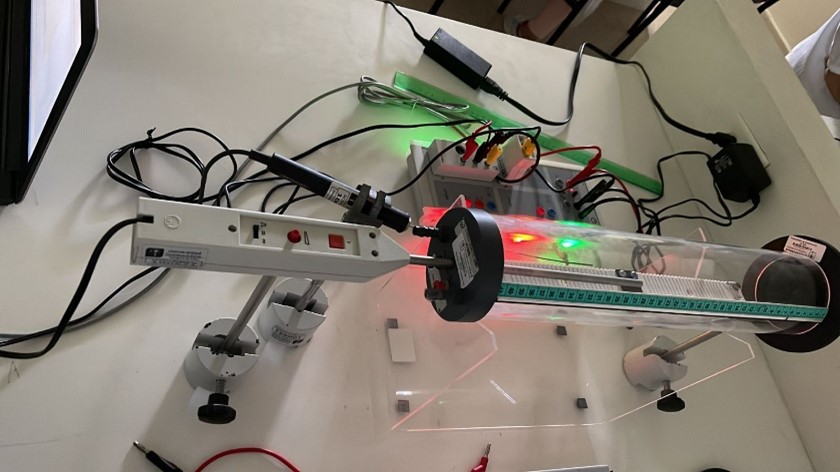
\includegraphics[width=\linewidth]{./Images/Imagen3.jpg}
    \caption{}
    \label{figure:me_1}
\end{figure}

\begin{figure}[H]
    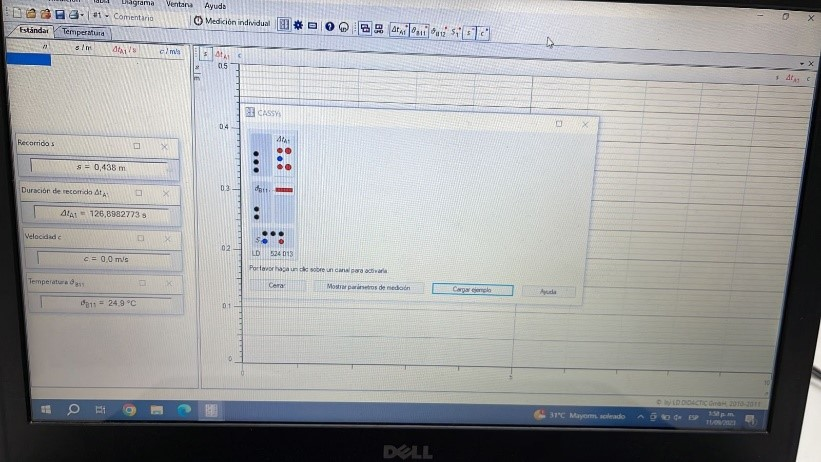
\includegraphics[width=\linewidth]{./Images/Imagen4.jpg}
    \caption{}
    \label{figure:me_2}
\end{figure}

Equipo utilizado:

\begin{itemize}
    \item Sensor\@{}-CASSY

    \item 1 Unidad Timer

    \item 1 Aparato para la medida de la velocidad del sonido.

    \item 1 Parlante para altas audiofrecuencias.

    \item 1 Micrófono universal.

    \item 1 Fuente de poder de 12 V, 3,5 A.

    \item 1 Regla metálica de 0,5 m.

    \item 1 PC con Windows 10 con el software CASSY Lab 2 preinstalado.
\end{itemize}

En el montaje que se muestra en la
figura~(\ref{figure:me_1}), para generar el sonido, movemos
la membrana del altavoz rápidamente usando una señal
eléctrica cuadrada. Este movimiento crea cambios en la
presión del aire dentro de un tubo. Para calcular la
velocidad del sonido (c), medimos el tiempo (t) que pasa
desde que generamos el sonido en el altavoz hasta que lo
detectamos con un micrófono. Donde se ven reflejados los
datos en software CASSY Lab 2 (~\ref{figure:me_2}), en el
cual a base de un promedio escogemos la medida dada.

% ! ----------------------------------------------------------------------|>
\section{Datos Experimentales}

\begin{table}[H]
    \begin{center}
        \begin{tabularx}{.9\linewidth}{|>{\centering\arraybackslash}X|>{\centering\arraybackslash}X|}
            \hline
            \multicolumn{2}{|c|}{Constantes}                         \\\hline
            $X_{1}$ \bolditalic{(m)}                     & $0,185$   \\\hline
            $t_{1}$ \bolditalic{(s)}                     & $0,00056$ \\\hline
            $T_{ambiente}$ \bolditalic{(°$\mathcal{C}$)} & $24,5$    \\\hline
        \end{tabularx}
    \end{center}
\end{table}

\begin{table}[H]
    \begin{center}
        \begin{tabularx}{.9\linewidth}{|>{\centering\arraybackslash}X|>{\centering\arraybackslash}X|}
            \hline
            $X_{2}$ \bolditalic{(m)} & $t_{2}$ \bolditalic{(s)} \\\hline
            $0,193$                  & $0,00054$                \\\hline
            $0,218$                  & $0,00065$                \\\hline
            $0,242$                  & $0,00072$                \\\hline
            $0,263$                  & $0,00078$                \\\hline
            $0,287$                  & $0,00086$                \\\hline
            $0,305$                  & $0,00092$                \\\hline
        \end{tabularx}
    \end{center}
\end{table}

\begin{table}[H]
    \begin{center}
        \begin{tabularx}{.9\linewidth}{|>{\centering\arraybackslash}X|>{\centering\arraybackslash}X|}
            \hline
            $\Delta t$ \bolditalic{(s)} & $c$ \bolditalic{(m/s)}  \\\hline
            $2,50000 \times 10^{-5}$    & $3,20000 \times 10^{2}$ \\\hline
            $9,00000 \times 10^{-5}$    & $3,66667 \times 10^{2}$ \\\hline
            $1,60000 \times 10^{-4}$    & $3,56250 \times 10^{2}$ \\\hline
            $2,20000 \times 10^{-4}$    & $3,54545 \times 10^{2}$ \\\hline
            $3,00000 \times 10^{-4}$    & $3,40000 \times 10^{2}$ \\\hline
            $3,60000 \times 10^{-4}$    & $3,33333 \times 10^{2}$ \\\hline
        \end{tabularx}
    \end{center}
\end{table}

\begin{table}[H]
    \begin{center}
        \begin{tabularx}{.9\linewidth}{|>{\centering\arraybackslash}X|>{\centering\arraybackslash}X|}
            \hline
            Promedio & $3,45133 \times 10^{2}$ \\\hline
        \end{tabularx}
    \end{center}
\end{table}

\vspace{-1cm}

\noindent\makebox[\linewidth]{\rule{.9\linewidth}{0.4pt}}

\begin{table}[H]
    \begin{center}
        \begin{tabularx}{.9\linewidth}{|>{\centering\arraybackslash}X|>{\centering\arraybackslash}X|}
            \hline
            \multicolumn{2}{|c|}{Constantes}                               \\\hline
            Distancia de viaje \bolditalic{(m)} & \multirow{2}{*}{$0,438$} \\\hline
        \end{tabularx}
    \end{center}
\end{table}

\begin{table}[H]
    \begin{center}
        \begin{tabularx}{.9\linewidth}{|>{\centering\arraybackslash}X|>{\centering\arraybackslash}X|}
            \hline
            $T$ \bolditalic{(°$\mathcal{C}$)} & $T$ \bolditalic{(°$\mathcal{K}$)} \\\hline
            $30$                              & $303,15$                          \\\hline
            $35$                              & $308,15$                          \\\hline
            $40$                              & $313,15$                          \\\hline
            $45$                              & $318,15$                          \\\hline
            $50$                              & $323,15$                          \\\hline
        \end{tabularx}
    \end{center}
\end{table}

\begin{table}[H]
    \begin{center}
        \begin{tabularx}{.9\linewidth}{|>{\centering\arraybackslash}X|>{\centering\arraybackslash}X|}
            \hline
            $t$ \bolditalic{(s)} & $c$ \bolditalic{(m/s)} \\\hline
            $0,0012507$          & $350,2038858$          \\\hline
            $0,0012235$          & $357,9893747$          \\\hline
            $0,0012193$          & $359,2225047$          \\\hline
            $0,0011972$          & $365,8536585$          \\\hline
            $0,0011860$          & $369,3086003$          \\\hline
        \end{tabularx}
    \end{center}
\end{table}

\begin{table}[H]
    \begin{center}
        \begin{tabularx}{.9\linewidth}{|>{\centering\arraybackslash}X|>{\centering\arraybackslash}X|}
            \hline
            Teorico \bolditalic{(m/s)} & Error \bolditalic{(\%)} \\\hline
            $349,268738$               & $0,2677$                \\\hline
            $352,137288$               & $1,6619$                \\\hline
            $354,982658$               & $1,1944$                \\\hline
            $357,805401$               & $2,2493$                \\\hline
            $360,606050$               & $2,4133$                \\\hline
        \end{tabularx}
    \end{center}
\end{table}

% ! ----------------------------------------------------------------------|>
\section{Análisis de datos}

% + -------------------------------------------------------------|>
\subsection{Análisis}

% * ------------------------------------|>
\subsubsection{}

La formula~(\ref{eq:velocidad_sonido_teorica}), es una
relación empírica que se utiliza para estimar la velocidad
del sonido en el aire a una temperatura $\mathcal{T}$.

La velocidad del sonido a temperatura ambiente
($24,5$\Celsius $= 297,65$ \Kelvin) es

\begin{equation*}
    c = (20,06)\sqrt{297,65} = 346,08 \frac{m}{s}
\end{equation*}

% * ------------------------------------|>
\subsubsection{}

% * ------------------------------------|>
\subsubsection{}

Velocidad promedio \hfill{} \break{} (Experimental) $=
    3,45113 \times 10^{2} \frac{m}{s}$

\smallskip

Velocidad teórica $= 346,08 \frac{m}{s}$

\smallskip

Porcentaje de error $= 0,00282\%$

% * ------------------------------------|>
\subsubsection{}

\begin{figure}[H]
    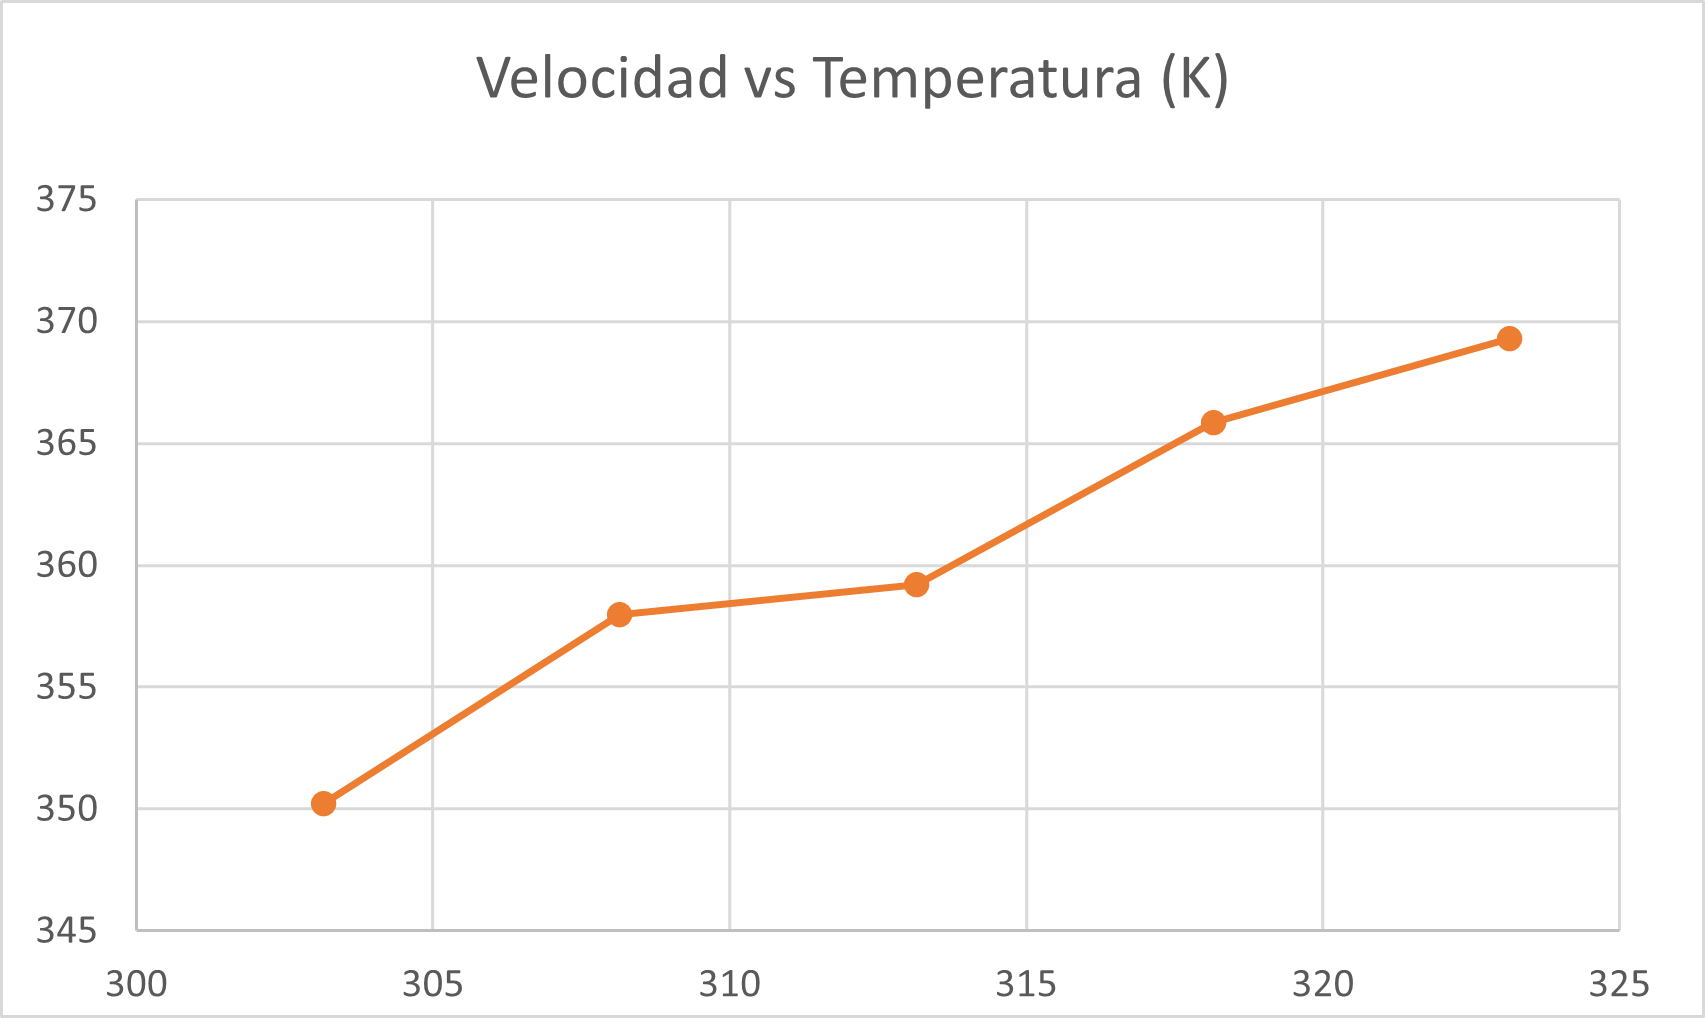
\includegraphics[width=\linewidth]{./Images/Imagen1.png}
    \caption{}
\end{figure}

\begin{figure}[H]
    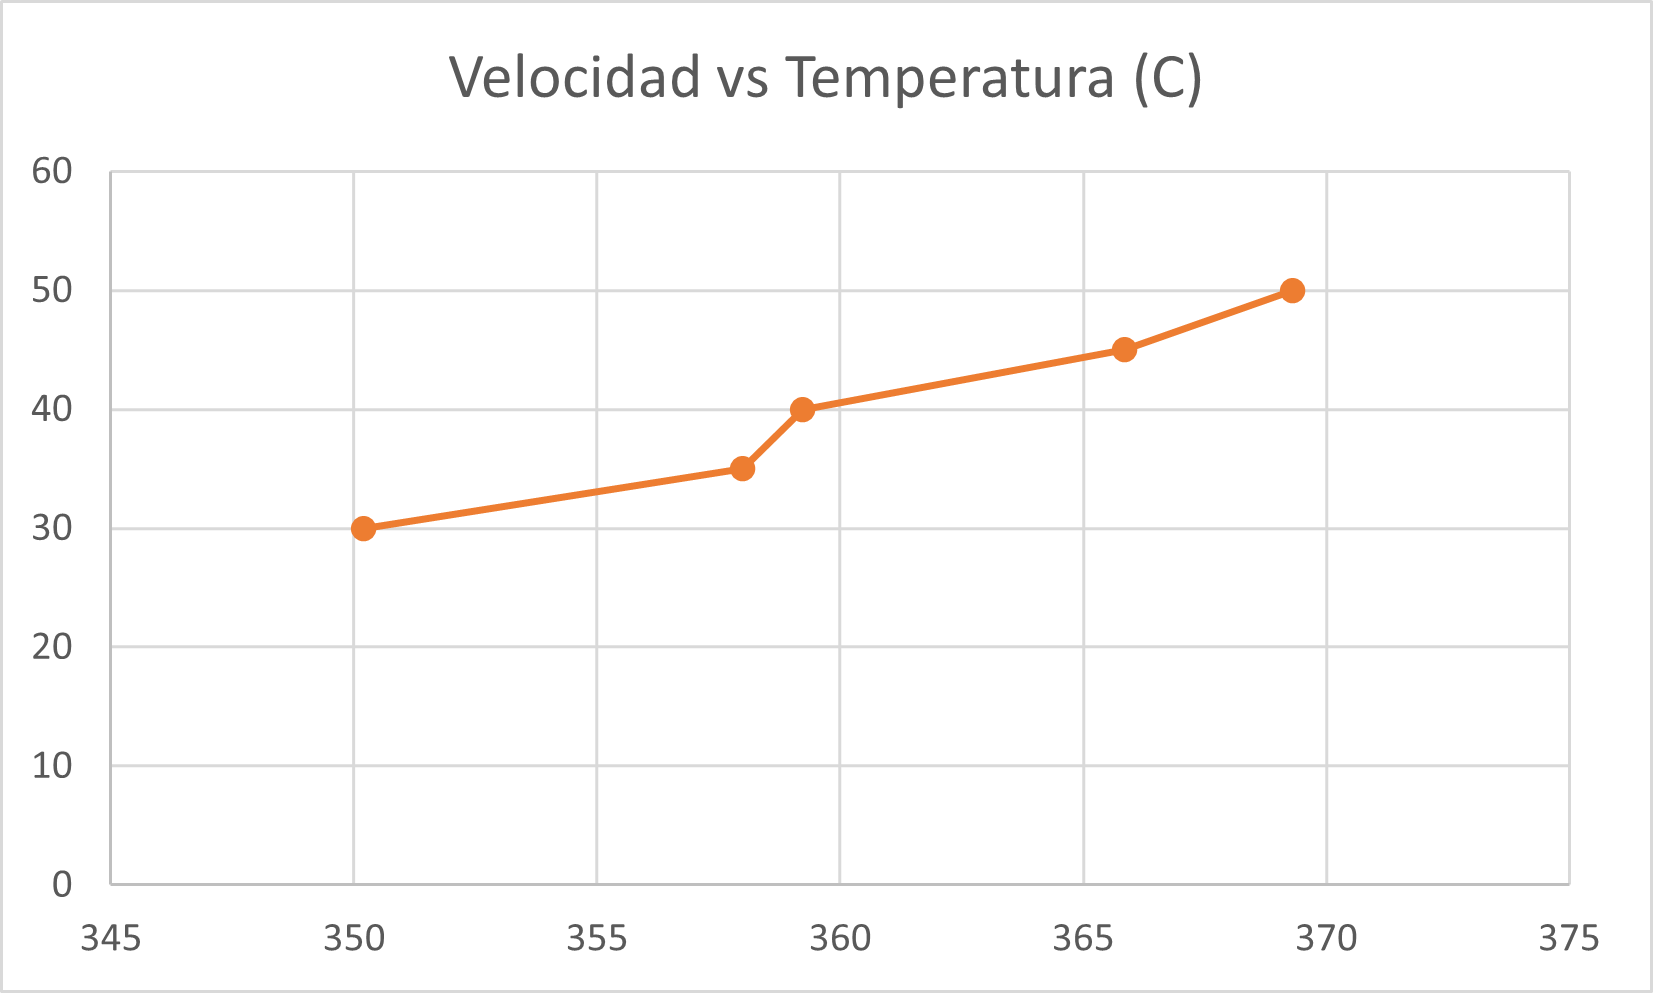
\includegraphics[width=\linewidth]{./Images/Imagen2.png}
    \caption{}
\end{figure}

% ! ----------------------------------------------------------------------|>
\section{Conclusiones}

En conclusión, este experimento demostró que la velocidad
del sonido en el aire está estrechamente relacionada con la
temperatura, siguiendo una dependencia directa. A medida
que la temperatura aumenta, la velocidad del sonido también
aumenta, lo que se puede explicar mediante la ecuación de
los gases ideales y la ecuación de onda de presión en los
gases. Además, el experimento destacó la importancia de
mantener la presión constante para aislar los efectos de la
temperatura en la velocidad del sonido. Estos resultados
son fundamentales para comprender cómo el sonido se propaga
en diferentes condiciones y son aplicables en diversos
campos, desde la acústica hasta la ingeniería.

\printbibliography

\end{document}